%! TEX program = pdflatex
\documentclass[a4paper,11pt]{article}

% Local packages
\usepackage{setup}
\usepackage{jheppub}

% TeXLive packages
%\usepackage{cite}
\usepackage{ifthen}
\usepackage{subcaption}
\usepackage{siunitx}
\usepackage{enumitem}
\usepackage{booktabs}
\usepackage{appendix}

% Bibliography
\bibliographystyle{JHEP}

% SI unit femtobarn
\DeclareSIUnit\fb{\femto\barn}

%% A few custom commands copied over from previous documents                     
\def \beq{\begin{equation}}
\def \eeq{\end{equation}}
\def \beqa{\begin{eqnarray}}
\def \eeqa{\end{eqnarray}}
\newcommand\numberthis{\addtocounter{equation}{1}\tag{\theequation}}

\def\nn{\nonumber }
\def\msbar{$\overline{\hbox{MS}}$}
\newcommand{\alert}[1]{{\bf \color{red}[{#1}]}} 
\def\bea{\begin{eqnarray}}
\def\eea{\end{eqnarray}}

\def\gsim{\mathrel{\rlap{\lower4pt\hbox{\hskip1pt$\sim$}}
    \raise1pt\hbox{$>$}}}         %greater than or approx. symbol
\def\lsim{\mathrel{\rlap{\lower4pt\hbox{\hskip1pt$\sim$}}
    \raise1pt\hbox{$<$}}}         %less than or approx. symbol


\begin{document}
\title{Notes on the calculation for neutrino-photon and neutrino-neutrino interactions.}

\author[1]{Rhorry}
\affiliation[1]{Max Planck Institute for Physics, Boltzmannstr. 8, 85748 Garching, Germany}
\emailAdd{rgauld@mpp.mpg.de}

\date{\today}
%\pacs{}

\abstract{A summary of the calculation of the various ingredients for neutrino-photon and neutrino-neutrino interactions is provided. This includes the computation of the squared amplitudes, phase-space setup, and implementation in a stand-alone c++ program.
%
Results for the behaviour of the cross-sections as a function of the centre-of-mass energy is also provided.
%
In the case of the production of QCD particles, the cross-section is computed assuming some lower invariant mass for the hadronic system (represented by the quarks).}

\maketitle
\flushbottom

\section{Introduction and notation}
Testing here the citation procedure~\cite{Gauld:2021zmq}.

In this document I summarise the computation of neutrino-photon and neutrino-neutrino scattering processes. This includes the computation of the squared amplitudes as well as the computation of the scattering process via numerical phase space integration.
%
These ingredients allow for a fully differential description of neutrino induced scattering on either CMB photons or neutrinos, which should hopefully allow for scattering and absorption effects in neutrino propagation to be studied.

I have tried to be exhaustive and consider all necessary channels for each process. Please let me know where things are missing and I can add them.

\paragraph{Neutrino-neutrino interactions.} For neutrino-neutrino scattering I have performed the 2to2 tree-level (LO) computation for the following channels,
\begin{enumerate}
	\item $\nu_1 + \bar{\nu}_1 \to f \bar f$
	\item $\nu_1 + \bar{\nu}_2 \to \nu_1 + \bar{\nu}_2$
	\item $\nu_1 + \nu_2 \to\nu_1 + \nu_2 + c.c.$
	\item $\nu_1 + \bar{\nu}_1 \to \nu_1 + \bar{\nu}_1$
\end{enumerate}
For the generic fermion final-state, the couplings and mass of the fermion are kept general. The resulting expressions are thus applicable to all SM fermions (with a factor of $n_c$ when considering quarks due to the colour sum). The subscript denotes the lepton flavour quantum number (e.g. electron type = 1, ..., etc.).

\newpage 
\paragraph{Neutrino-photon interactions.} For neutrino-photon scattering I have performed the 2to3 tree-level (LO) computation for the following channels (code name in parenthesis)
\begin{enumerate}
	\item $\nu_1 + \gamma \to \nu_1 + {\rm quarks}$ ($\nu_1q\bar q$)
	\item $\nu_1 + \gamma \to \ell_1 + {\rm quarks}$ ($\ell_1q\bar q^{\prime}$)
	\item $\nu_1 + \gamma \to \nu_1 + {\rm leptons, flavour\neq1}$ ($\nu_1 \ell_2 \bar\ell_2$)
	\item $\nu_1 + \gamma \to \ell_1 + {\rm leptons, flavour\neq1}$ ($\ell_1 \nu_2 \bar\ell_2$)
	\item $\nu_1 + \gamma \to \ell_1 + {\rm leptons, flavour=1}$ ($\ell_1 \nu_1 \bar\ell_1$)
\end{enumerate}
In these computations the neutrino mass is always neglected, the charged lepton masses are retained, and the quark masses have been retained (except in case 2.). Note that since the quark masses regulates a $\gamma \to q \bar q$ collinear singularity, some care is needed for the quark computation when integrating over phase-space. Finally, when considering lepton production, one must consider the cases when the flavour of the outgoing lepton may be the same/different as the incoming neutrino flavour. Those are differentiated through the flavour subscripts.

\section{Computation of squared amplitudes}

\subsection{neutrino-neutrino interactions}
These computations are the most simple. They are performed while keeping the masses general, the couplings of the fermions complex (to allow for use in arbitrary EW input schemes), complex propagators, and then implemented in the code.

The results for these squared amplitudes are accessed through the master function \verb|ME2_nu1nu2_ffx({p},i,j,k,l)|, where the set $\left\{p\right\}$ contains the four-momenta momenta of the particles and the integers $i,j,k,l$ are the PDG labels of the particles.
%
The integers $i,j$ should correspond to (anti)neutrinos (-)12,(-)14,(-)16, while the outgoing fermions should be either neutrinos, or in the special case of neutrino annihilation to fermions of $i = -j$ and $k = -l$.

The various results for each channel are implemented explicitly in functions like: \verb|ME2_nu1nu1x_ffx|, \verb|ME2_nu1nu2_nu1nu2|, which are then accessed via the master function.

\subsection{neutrino-photons interactions}
The 2to3 neutrino-photon computations are more involved (some channels have 10 feynman diagrams), and obtaining some compact analytic results took more care.

\begin{figure}[ht]
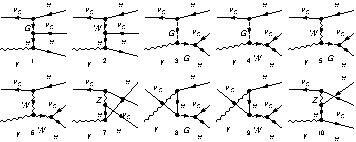
\includegraphics[width=1.0\textwidth]{Diagrams-crop.pdf}
\caption{Sample of the Feynman diagrams in the most complicated channel involving all same flavour leptons.}
\label{fig:diagrams}
\end{figure}

It will be useful to introduce some notation for the full amplitude corresponding to the sum of all diagrams in Fig.~\ref{fig:diagrams}.
%
The full amplitude (including both $\PZ$ and $\PW$ bosons exchanged --- and their corresponding Goldstone bosons contributions) may be written
\beq
\mathcal{M} = \mathcal{M}_Z + \mathcal{M}_W
\eeq
%
The part of the amplitude involving only $\PZ$ bosons would be diagrams 7 and 10. These make up $\mathcal{M}_Z$, while the rest form $\mathcal{M}_W$.


\paragraph{$\nu_1 q\bar q$ and $\nu_1 \ell \bar \ell$.}
The most simple computation are the $\nu_1 q\bar q$ (1) and $\nu_1 \ell \bar \ell$ (3) channels which involve the neutrino line which couples to the electromagnetically charged fermion line (either quark or lepton). The analytic results for these channels are related to one another by a factor of $n_c$ and a charge factor of $Q_f^2$. These correspond to diagrams of type 7 and 10 in Fig.~\ref{fig:diagrams}, and the squared amplitude is simply $|\mathcal{M}_Z|^2$.
%
The analytic result is implemented in the function \verb|ME2_nugam_nuffx({p},i,j,k,l,m)| 

\paragraph{$\ell_1q\bar q^{\prime}$.}
This computation is quite a bit more complicated and involves the $WW\gamma$ vertex (which makes the treatment of the \PW boson width effects more complicated). This computation has been performed neglecting the outgoing quark masses and includes the complex mass effects in the propagators. To have this squared amplitude exact in the complex mass scheme I may need to revisit the treatment of complex couplings. It has been validated in the $\Gamma_W \to 0$ and $m_{\ell}\to0$ limit against a similar amplitude in OpenLoops to 15 digits. When all width effects are included in OpenLoops, the agreement is typically 1per mille for some random phase space points I generated. These correspond to diagrams in Fig.~\ref{fig:diagrams}, but excluding type 7 and 10, and the squared amplitude is simply $|\mathcal{M}_W|^2$.

\paragraph{$\ell_1 \nu_2 \bar\ell_2$.}
This computation is the same as the one above, except that the mass of the fermion $\ell_2$ is retained.

\paragraph{$\ell_1 \nu_1 \bar\ell_1$.}
By far the most complicated case is that when the flavour of the outgoing leptons are identical.
%
In this case the contributing Feynman diagrams are all of those shown in Fig.~\ref{fig:diagrams}.
%
The previous computations are actually a subset of these. To obtain the result in this channel, one can observe that the amplitude will have the form
%
\beq
\mathcal{M} = \mathcal{M}_Z + \mathcal{M}_W
\eeq
%
where the subscript denotes the diagrams which involves the $\PZ$ or $\PW$ boson (or the corresponding Goldstone boson). The total result for the squared amplitude is therefore
%
\beq
|\mathcal{M}|^2 = |\mathcal{M}_Z|^2 + |\mathcal{M}_W|^2 +\mathcal{M}_Z \mathcal{M}_W^{\dagger} + \mathcal{M}_W \mathcal{M}_Z^{\dagger}
\eeq
%
The result for $|\mathcal{M}_Z|^2$ and $|\mathcal{M}_W|^2$ are simply those for the channels $\nu_1 \ell \bar \ell$ and $\ell_1 \nu_2 \bar \ell_2$ discussed above, and what is missing is the additional interference terms.
%
Thus I compute directly the interference terms 
%
\beq
\mathcal{M}^2_{\rm inter.} = \mathcal{M}_Z \mathcal{M}_W^{\dagger} + \mathcal{M}_W \mathcal{M}_Z^{\dagger}
\eeq
and make use of the existing results for the simpler cases.

\alert{In this case I was only able to obtain a result making the assumption of real valued couplings. This means for a complex mass scheme, there are width effects missing in the computation. Typically these are permille effects and thus not relevant for the cross-section result. I may try revisit this later.}

\section{Cross-section and phase space implementation}
The scattering computation is generally performed according to
%
\beq
{\rm d} \sigma = \frac{1}{2 \hat{s}} \overline{\sum} |\mathcal{M}|^2 {\rm d}\Phi_n
\eeq
%
which includes the flux factor, the summed/averaged squared amplitude, and the final-state phase space. 
%
The flux factor is trivially $\hat{s} = s_{12} = 2 p_1 \cdot p_2$ for massless incoming particles (the photon and neutrino[s]), and the squared amplitudes have been discussed in the previous section.
%
The approach taken in the sample c++ code (and which should also be used in the propagation code) is to implement the fully differential phase-space and then perform the integration numerically. The benefit of this approach is that we can easily define the four-momenta of all incoming/outgoing particles for every single integrand point (i.e. a phase space point). In otherwords, we will always have access the four momenta of the scattered particles we are interested in.

To achieve this one can use the general formula for a two-body phase space for outgoing particles with momenta $p_i$ and $p_j$ in the $p_{ij} = p_i + p_j$ rest frame:
%
\beq
{\rm d}\Phi_2(m_{ij}^2;p_i,p_j) = \frac{\rm d \cos \theta d \phi}{2(4\pi)^2} \lambda^{1/2}\left(1,\frac{m_i^2}{m_{ij}^2},\frac{m_j^2}{m_{ij}^2}\right)\,,
\eeq
%
with $\lambda$ the Kallen function.
%
For 2to2 scattering the $d\phi$ integration is performed analytically (since $|\mathcal{M}|^2$ does not depend on it).

For the three-body final state we make use of the factorisation formula
%
\beq
{\rm d}\Phi_3(m_{ijk}^2;p_i,p_j,p_k) = {\rm d}\Phi_2(m_{ijk}^2;p_i,p_{jk}) \frac{d m_{jk}^2}{2 \pi} {\rm d}\Phi_2(m_{jk}^2;p_j,p_k)\,.
\eeq
%
The first 2-body phase integral (involving particle $i$ and the composite system $jk$) is performed in the centre-of-mass energy ($ijk$ frame), while the phase-space integration of the $jk$ sub-system is performed in the $jk$ rest frame. One simply must boost the particle momenta $j$ and $k$ to the $ijk$ rest frame, and then all momenta to the CMB frame.
%
This is convenient for us, since the integration limits are extremely simple in this case, and the required Lorentz boosts are applied numerically.

\section{Results}

\bibliography{NeutrinoScattering}

\end{document}
